\section{Evaluation}
\label{sec:sdwodeval}

To evaluate our system, we wanted to measure the accuracy of the matches, in a real-world set-up, with real data. We only evaluate the matching component of the system, since the query component is straightforward and its performance depends on external factors, like the availability of the services used and the network connection.
To assess the results of the matching, we created two entity corpora, one with desktop data and one with Web data. On these corpora, we first created a baseline from relevance judgements made by human experts. Then, we ran our entity matching algorithm and we computed precision, mean average precision (MAP), and normalised discounted cumulative gain (NDCG) to measure its performance. 

\subsection{Data Collection}

We created two corpora for the evaluation, one containing desktop entities, and one containing possible matching entities from the Web of Data. The Web corpus was obtained by using the query component of the system, with the only active plugin being the Sindice one.

\subsubsection{Desktop data entity corpus}

The desktop data used in the evaluation was collected from a real, in-use Nepomuk-KDE Semantic Desktop. It was generated by Nepomuk applications, and extracted from the desktop repository.

We restricted the entities selected to three types: 
\begin{itemize}
 \item people --- of type \verb|nco:PersonContact|, 
 \item publications --- of type \verb|nfo:PaginatedTextDocument|, and 
 \item music albums --- \verb|nmo:MusicAlbum|.
\end{itemize} 
From each type we collected fifty distinct resources, resulting in a corpus of 150 seed desktop entities, and other entities related to them. Examples of auxiliary entities are the authors of publications, which may or may not be already in the corpus as contacts, the tracks of the albums and the artists. In total the desktop data corpus has 11,917 triples.

We used information from our desktops, therefore the people are colleagues or other researchers we collaborate with; the publications are related to our research interests, and generally related to semantics and information extraction. The music albums data was gathered from several colleagues, for variety of genres.

The contact data is extracted by Nepomuk from the default KDE address book application, and we made no changes to it. The correct way to use the \verb|nco:PersonContact| resources extracted automatically, is to link each of them to a corresponding \verb|pimo:Person| representing the person who has the contact information. However, the current tools do not make the distinction, therefore we also used the ``raw'' \verb|nco:PersonContact| resources, for simplicity. The algorithm makes no distinction between types, so it would yield identical results if we had used the ``proper'' \verb|pimo:Person|.  

The information related to music albums is extracted automatically by Nepomuk from the ID3 tags of music files. 

For publications we used Sclippy\footnote{\url{http://smile.deri.ie/projects/sclippy}}, an existing tool described in \cite{Groza2009}, to perform shallow metadata extraction from files to obtain the title and the authors of the publications, when the metadata of the documents was not set.

\subsubsection{Web of Data entity corpus}

We used the query module of our system to generate the second corpus, containing Web of Data entities. More precisely, we used the Sindice plugin to retrieve the first twenty results returned by Sindice, for each desktop entity, thus making a total of 3,000 URIs. The queries used in Sindice were constructed as presented in Section~\ref{sub:querymodule}, a combination based on the properties of each desktop entity. For each URI we obtained all the triples extracted by Sindice --- explicit and implicit. In total this corpus has 1,530,686 triples.

In this dataset we did not explicitly retrieve Sindice data for the auxiliary entities related to the result URIs. We assumed that this data will be available when and if required --- in the relevance judgements by experts, and in the matching process by the algorithm.

\subsection{Relevance Judgements from Experts}

We collected the relevance judgements from experts through an online experiment, in which we asked participants to decide if pairs of desktop and Web URIs identify the same real-world object or person. We evaluated in this way all 3,000 pairs from the two corpora. Each pair was judged by three different experts. Eighteen people participated in the experiment, all researchers in the area of Semantic Web. 

To simplify the task, we presented the two entities side by side, with all the information which was available about them in the corpora (see Figure~\ref{fig:onlineexperiment}). The desktop entity is shown on the left, and the Web entity on the right. On the Web side we included hyperlinks to the related entities, for further exploration in case the information given was not sufficient for making the decision. For convenience, on the Web side, we have separated and brought to the top the triples which partially matched any of the values from the desktop side. 

\begin{figure}[htb]
 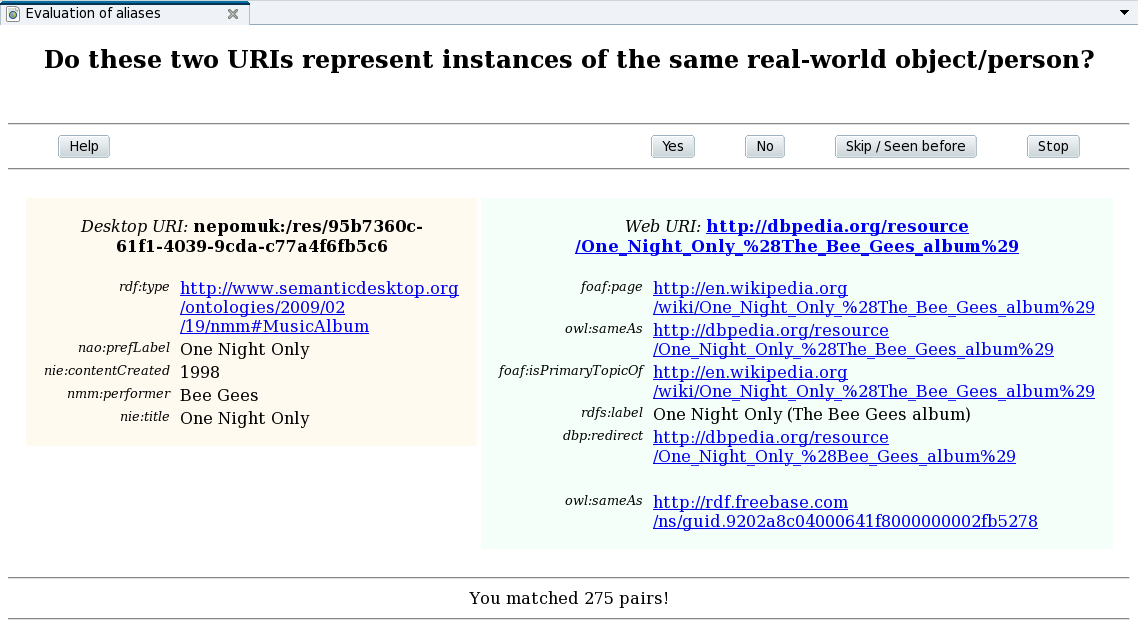
\includegraphics[width=\linewidth]{chapters/core/img/eval_album.png}
\caption{The Web interface of the experiment for collecting relevance judgements.}
\label{fig:onlineexperiment}
\end{figure} 

There were only two decisions possible: \emph{Yes} or \emph{No}, with a \emph{Skip} option, in case of uncertainty. Once a pair was judged or skipped, another one was shown to the participant. The pairs were randomly chosen from the remaining set. To add a gamification element to the experiment, we kept count of the number of pairs judged by each participant, and displayed it on the page. We found that even such a small addition generated ad-hoc competition and made the dull task more interesting.

The results of the experiment show an average agreement and its standard deviation, computed with Fleiss's $\kappa$, of $0.638\pm0.214$, over all three types of entities, suggesting substantial agreement between annotators. Table~\ref{tab:agreementsdwod} shows the Fleiss's $\kappa$ and its standard deviation $\sigma$ per type, as well as the average pairwise percent agreement. We observed that for music albums, there was only moderate agreement between annotators, visibly lower than the average, while for publications it is visibly higher. We believe the difference is caused by the fact that the data about publications is generated and curated by experts in the field --- even more so, as the publications were largely from the domain of Semantic Web --- while the music data comes from much more heterogeneous sources.

\begin{table}
\centering
\ra{1.3}
\begin{tabular}{@{}rcl@{\hs}l@{\hs}l@{}}
\toprule
& \phantom{a} & $\kappa$ & $\sigma$ & Avg  \\ 
\midrule

 All && 0.638 & 0.214 & 92.252 \\

 People && 0.661 & 0.257 & 88.2 \\

 Publications && 0.786 & 0.127 & 98.067  \\

 Albums && 0.442 & 0.233 & 90.523 \\

\bottomrule
\end{tabular}
\caption{Inter-annotator agreement measures}
\label{tab:agreementsdwod}
\end{table}

\subsection{Quantitative Results}

To evaluate the performance of the algorithm, we evaluate each of the matching parameters described in Section \ref{sub:matchingcomp}, activated either separately or using a combination of them, against a baseline which is the matching framework with all the parameters disabled. In the following, the String Matching parameter is denoted by SM, the Weighted Properties by WP and the Multi-Valued Properties by MVP.

We used the \emph{trec\_eval} tool\footnote{\url{http://trec.nist.gov/trec_eval/}} to compute standard information retrieval measures.
The precision at k ($P@k$) with k={1,2,3,4,5}, mean average precision (MAP) and normalised discounted cumulative gain (NDCG) are reported in Table~\ref{tab:agreement-albums} for music albums, Table~\ref{tab:agreement-people} for people and Table~\ref{tab:agreement-publications} for publications. 
We report also the interpolated precision at recall cut-off points when all matching parameters are enabled. The goal for the system is high precision, i.e., achieving a maximum at P@1. Recall is not a target, as it is generally impossible to determine the entire set of correct results available in the Web of Data.

\begin{table}[htb]
\centering
\ra{1.3}
\begin{tabular}{@{}rcl@{\hs}l@{\hs}l@{\hs}l@{\hs}l@{\hs}l@{\hs}l@{}}
\toprule
& \phantom{a} & MAP & NDCG & P@1 & P@2 & P@3 & P@4 & P@5 \\ 
\midrule

 SM WP MVP && 0.2464 & 0.5117 & 1 & 0.625 & 0.4167 & 0.3125 & 0.25 \\ %111

 SM WP && 0.2464 & 0.5117 & 1 & 0.625 & 0.4167 & 0.3125 & 0.25 \\ %110

 SM MVP && 0.2464 & 0.5117 & 1 & 0.625 & 0.4167 & 0.3125 & 0.25 \\ %101

 WP MVP && 0 & 0 & 0 & 0 & 0 & 0 & 0 \\ %011

 SM && 0.2464 & 0.5117 & 1 & 0.625 & 0.4167 & 0.3125 & 0.25 \\ %100

 WP && 0 & 0 & 0 & 0 & 0 & 0 & 0 \\ %010

 MVP && 0 & 0 & 0 & 0 & 0 & 0 & 0 \\ %001

 Baseline && 0 & 0 & 0 & 0 & 0 & 0 & 0 \\ %000

\bottomrule
\end{tabular}
\caption{Evaluation results for albums, when varying configuration parameters.}
\label{tab:agreement-albums}
\end{table}

In Table~\ref{tab:agreement-albums}, we can observe that only the SM parameter is enhancing the results compared to the baseline. The other two parameters do not improve the results at matching certain candidates. Also, in term of MAP and NDCG, the system achieves the lowest performance on the albums corpus. This can be explained by the fact that the Web resources returned by the query module for albums are mostly e-commerce products, which are not defined as a type of interest, and therefore are rejected by the matching module. However, some of the annotators have considered that the corresponding candidates are indeed the same as the album, while some have disagreed --- this is reflected in the agreement measure, as for the albums we have the lowest value for Fleiss's $\kappa$. Whether or not such candidates should have been kept by the system is open to discussion and left for future work.

\begin{table}[htb]
\centering
\ra{1.3}
\begin{tabular}{@{}rcl@{\hs}l@{\hs}l@{\hs}l@{\hs}l@{\hs}l@{\hs}l@{}}
\toprule
& \phantom{a} & MAP & NDCG & P@1 & P@2 & P@3 & P@4 & P@5 \\ 
\midrule

 SM WP MVP && 0.4212 & 0.6354 & 0.9302 & 0.8953 & 0.7597 & 0.6337 & 0.5442 \\ %111

 SM WP && 0.4174 & 0.6321 & 0.9286 & 0.8929 & 0.746 & 0.6131 & 0.5286 \\ %110

 SM MVP && 0.4212 & 0.6354 & 0.9302 & 0.8953 & 0.7597 & 0.6337 & 0.5442 \\ %101

 WP MVP && 0.2916 & 0.5338 & 1 & 0.8243 & 0.6036 & 0.473 & 0.3838 \\ %011

 SM && 0.4212 & 0.6354 & 0.9302 & 0.8953 & 0.7597 & 0.6337 & 0.5442 \\ %100

 WP && 0.2916 & 0.5338 & 1 & 0.8243 & 0.6036 & 0.473 & 0.3838 \\ %010

 MVP && 0.2877 & 0.53 & 1 & 0.8243 & 0.6036 & 0.4662 & 0.3784 \\ %001

 Baseline && 0.2877 & 0.53 & 1 & 0.8243 & 0.6036 & 0.4662 & 0.3784 \\ %000

\bottomrule
\end{tabular}
\caption{Evaluation results for people, when varying configuration parameters.}
\label{tab:agreement-people}
\end{table}

In Table~\ref{tab:agreement-people}, we can observe that the baseline, the WP and the MVP parameters are each able to match good candidates with high precision at P@1, with WP providing slightly better MAP and NDCG. However, the system does not get significant advantage by combining them. The SM parameter alone provides slightly lower precision at P@1 but significantly better MAP and NDCG. By combining the three parameters, the system does not get significant advantage and it seems that using SM prevails. 

\begin{table}[htb]
\centering
\ra{1.3}
\begin{tabular}{@{}rcl@{\hs}l@{\hs}l@{\hs}l@{\hs}l@{\hs}l@{\hs}l@{}}
\toprule
& \phantom{a} & MAP & NDCG & P@1 & P@2 & P@3 & P@4 & P@5 \\ 
\midrule

 SM WP MVP && 0.7773 & 0.8651 & 1 & 0.625 & 0.4167 & 0.3125 & 0.25 \\ %111

 SM WP && 0.8032 & 0.8609 & 0.9062 & 0.5781 & 0.3958 & 0.3047 & 0.2438 \\ %110

 SM MVP && 0.7175 & 0.7986 & 0.9231 & 0.5769 & 0.3846 & 0.2885 & 0.2308 \\ %101

 WP MVP && 1 & 1 & 1 & 0.5 & 0.3333 & 0.25 & 0.2 \\ %011

 SM && 0.7265 & 0.7883 & 0.8235 & 0.5294 & 0.3627 & 0.2868 & 0.2294 \\ %100

 WP && 0.6893 & 0.7347 & 1 & 0.55 & 0.3667 & 0.275 & 0.22 \\ %010

 MVP && 0 & 0 & 0 & 0 & 0 & 0 & 0 \\ %001

 Baseline && 0.7175 & 0.7588 & 1 & 0.5455 & 0.3636 & 0.2727 & 0.2182 \\ %000

\bottomrule
\end{tabular}
\caption{Evaluation results for publications, when varying configuration parameters.}
\label{tab:agreement-publications}
\end{table}

In Table~\ref{tab:agreement-publications}, the baseline provides good results from the start for publications. The system is not able to return any candidates when MVP alone is activated. However, when WP and MVP are combined, the system achieves much better results (in term of MAP and NDCG) than the baseline or than the WP parameter alone. When the system combines SM with the two previous ones, the system achieves a lower MAP and NDCG but an improved precision with a larger cut-off rank. While on the two previous types of entities, the SM parameter seemed to be the most important matching feature, this corpus shows that the WP and MVP are important matching features in certain cases.

\begin{figure}[htb]
 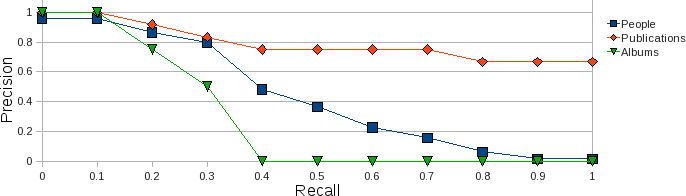
\includegraphics[width=\linewidth]{chapters/core/img/precrecal_wlabels.png}
\caption{Interpolated precision at recall cut-off points.}
\label{fig:precrecall}
\end{figure}

Overall, the results are satisfying for our use cases where high precision prevails over recall. However, given the results shown in Figure~\ref{fig:precrecall}, we can see that the system could be configured to return more than one entity in order to achieve better recall while keeping good precision. It might prove useful to implement a semi-automatic system which presents the top \emph{n} candidates to the user for manual selection.

\subsection{Performance}

To determine the performance, we measured the time spent on each step of the algorithm. We note that these results come from a prototype implementation, still to be subject to technical optimisations. Table~\ref{tab:sdwodtimes} shows the average times overall, and for each resource type separately, when all three parameters (SM, WP, MVP) are active. We find only small variations in the measurements when the parameter values are changed. We do not consider the time spent on retrieving data from Sindice, as this depends on external factors, like network speed and server availability. 

\begin{table}[htb]
\centering
\ra{1.3}
\begin{tabular}{@{}rcr@{\hs}r@{\hs}r@{\hs}r@{}}
\toprule
& \phantom{a} & Overall & People & Publications & Albums \\ 
\midrule

 Pair total && 375.04 & 52.19 & 977.87 & 53.18 \\

 Types check && 0.23 & 0.26 & 0.21 & 0.23 \\

 Per property check && 6.66 & 0.92 & 13.2 & 22.06 \\

 All properties && 2026.22 & 7.17 & 5478.87 & 1963.88 \\

\bottomrule
\end{tabular}
\caption{Time performance (milliseconds).}
\label{tab:sdwodtimes}
\end{table}

The checking of types is the only value that on average does not depend on the type of resource, as it must be performed for all pairs. The time spent in average per property check is low, but it varies by type, and by the complexity of the properties (e.g. it takes longer if several resources in the graph must be traversed, for long property paths like the name of the artist of an album). The ``All properties'' row shows the average time required for checking all the properties of an entity, and the computation of the final score\footnote{The ``All properties'' row has values higher that the ``Pair total'' row because the average time is computed only for those pairs that passed the type check, thus fewer, but with longer computation times.}. These values depend on the type of resources as well, and on the complexity of the resource graph. We found that longer times correspond to very big graphs for online entities, which must be loaded for checking even if in most cases are not found to represent valid 
candidates\footnote{e.g., the graph for \url{http://webconf.rkbexplorer.com/models/iswc-aswc-2007-complete.
rdf}}.
